
\documentclass[12pt]{article}
\usepackage{amsmath,amssymb,pdfpages,graphicx}
\begin{document}

\begin{center}
\section*{Numerical Solver for Time Independent Schr\"odinger Equation}
Zachary Faber Manning, Remy Wang, Erick Orozco
\end{center}

Time Independent Schrodinger Equation
\begin{equation}
-\frac{1}{2}\psi(x) + V(x)\psi(x) = E\psi(x)
\end{equation}
where $V(x)$ is the potential function

\bigbreak
We will be testing a solver using a potential function

\begin{equation}
\begin{array}{ll}
V(x) = 
\begin{cases}
\infty & x \leq 0 ,\\
x & x > 0
\end{cases}
\end{array}
\end{equation}

\bigbreak
This forms the resultant differential equation on the interval $(0, \infty)$
\begin{equation}
-\frac{1}{2}\psi(x) + x\psi(x) = E\psi(x)
\end{equation}

This ODE was discretized in the following manner:
\begin{equation}
u_{i+1} = u_i - 2(E\psi - x\psi)
\end{equation}
\begin{equation}
\psi_{i+1} = \psi_i + udx
\end{equation}
where $u=\psi'$

\bigbreak

Given an energy, $E$, and a maximum length, $l$, the solver first determines the wavefunction on the interval $(0,l)$. Starting with the initial conditions $(x, \psi, \psi') = (0, 0, 1)$, the solver iterates based on the above discretized form of the Schr\"odinger equation. This continues until a value of $x = l$ is reached, at which point the final value of the wavefunction, $\psi(l)$ is recorded.

\bigbreak

This process is repeated over intervals of $E$ and $l$, resulting in a series of functions of $\psi(l, E)$ where $l$ is the maximum length of integration, and $\psi$ is the final value of the wavefunction recorded at this length. The roots of this function at any given $l$ represent the series of energy eigenvalues of the potential function
\begin{equation}
\begin{array}{ll}
V(x) = 
\begin{cases}
\infty & x \leq 0 ,\\
x & 0 < x < l,\\
\infty & x \geq l
\end{cases}
\end{array}
\end{equation}

Thus, $\lim_{l \to \infty}\psi(l, E)$ has roots corresponding to the energy eigenvalues of the original potential function (2).

\bigbreak

The two root-finding methods we use are Newton's and Bisect. Below, is a figure that shows a $\psi$ at a specific $l$ with varying E values.

\begin{center}
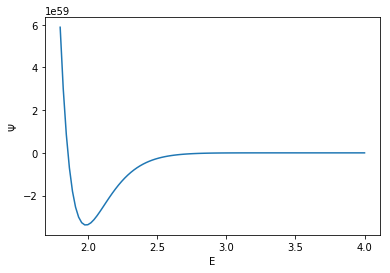
\includegraphics{psilOverE.png}
\end{center}

The root-finder determines a series of eigenvalues for which $\psi(l) = 0$. When iterated over a series of values of $l$, the eigenvaleus converge.

\bigbreak
\bigbreak

For Newtown's method:
\begin{center}
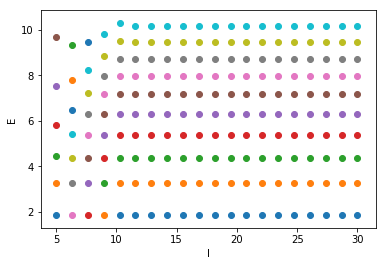
\includegraphics{newtonEigen.png}
\end{center}

As clearly shown, as $l$ approaches zero, the eigenvalues diverge, and as $l$ increases, the eigenvalues neatly converge. 

\bigbreak
\bigbreak
\bigbreak
\bigbreak
\bigbreak
\bigbreak
\bigbreak
\bigbreak
\bigbreak
\bigbreak
\bigbreak
\bigbreak
\bigbreak
\bigbreak
\bigbreak
\bigbreak
\bigbreak
\bigbreak
\bigbreak
\bigbreak

For the Bisect method:
\begin{center}
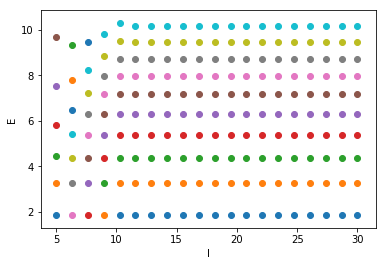
\includegraphics{bisectEigen.png}
\end{center}
 
Extremely similar to Newton's method's results, but the run time was significantly longer.

\bigbreak

Corresponding to these eigenvalues, we can determine a series of valid wavefunctions using our discretized equations, (4) and (5).

\begin{center}
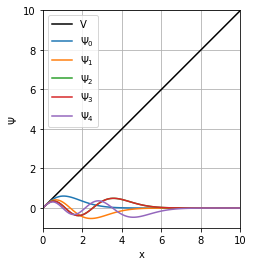
\includegraphics{psiNotNorm.png}
\end{center}

\bigbreak

These functions can be modified to satisfy the normalization equation, 
\begin{equation}
\int_{-\infty}^{\infty}|\psi|^{2}dx = 1
\end{equation}
so that the probability of observing the particle on the interval $(-\infty,\infty)$ is 1. By finding this integral for our current wavefunctions, we can find a scalar $c$ such that
\begin{equation}
c\int_{-\infty}^{\infty}|\psi|^{2}dx = 1
\end{equation}
holds for each function, and scale them accordingly. This yields the following normalized wavefunctions:

\begin{center}
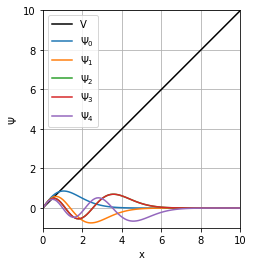
\includegraphics{psiNormalized.png}
\end{center}

\bigbreak

Using Mathematica, we came to the following analytical solutiion for $\psi(x)$:

\begin{equation}
\psi(x) = AiryAi[2^{1/3}(x-E)]C_{1} + AiryBi[2^{1/3}(x-E)]C_{2}
\end{equation}

This Airy equation nonsense is new to us since we've never taken quantum theory before. However, we understand that it is utilized to solve Schr\"odinger's equation thanks to Wikipedia.

\end{document}
